\documentclass[11pt,compress,t,notes=noshow, xcolor=table]{beamer}


\input{../../style/preamble}
\input{../../latex-math/basic-math}
\input{../../latex-math/basic-ml}

\title{Optimization in Machine Learning}

\begin{document}

\titlemeta{% Chunk title (example: CART, Forests, Boosting, ...), can be empty
  First order methods
  }{% Lecture title  
  Comparison of first order methods
  }{% Relative path to title page image: Can be empty but must not start with slides/
  figure_man/linesearch.png
  }{
    \item Gradient Descent
    \item Stochastic Gradient Descent
    \item Momentum
    \item Step size decay
}


\begin{vbframe}{Comparison of first order methods}
Comparison of (S)GD, (S)GD + momentum, and (S)GD + momentum + step size control on simulated data. We do not use analytical solution on purpose although one exists:
{\small
\begin{itemize}
    \item Linear regression (squared loss) simulation $\bm{y} = \bm{X}\thetav^{\ast} + \bm{\varepsilon}$ with $n=500$ samples and $p=11$ features, where $\thetav^{\ast}=(-5,-4,\ldots0,\ldots,4,5)^{\top}$, $\bm{\varepsilon} \sim \mathcal{N}(\bm{0}, \bm{I})$, and $\bm{X} \sim \mathcal{N}(\bm{0}, \Sigma)$ for $\Sigma=\bm{I}$ (i.i.d. features) or $\Sigma_{i,j}=0.99^{|i-j|}$ (corr. features)
    \item Indep. features result in a condition number of $\approx 2.9$, whereas the corr. feature set-up produces a (moderately) bad condition number of $\approx 600$
    \item We set the momentum parameter to $0.8$ and the decay step size using schedule $\alpha^{[t]}=\alpha^{[0]} \cdot \texttt{decay}^{t/t_{\text{max}}}$ for $\texttt{decay}=0.1$
    \item For GD and SGD we use different step sizes to show that benefit of momentum/decay depends heavily on step size
    \item ERM has unique global minimizer given by $\bm{\thetah} = (\bm{X}^{\top}\bm{X})^{-1}\bm{X}^{\top} \bm{y}$
    \item We also track the optimization error $\Vert \thetav - \bm{\thetah} \Vert_2$
\end{itemize}
}
\end{vbframe}

%%%% GD linear

\begin{vbframe}{Lin-Reg (GD + med step size, default case)}
\vspace{-0.4cm}
GD with medium $\alpha=2\cdot10^{-3}$ and indep. features:
\begin{figure}
            \includegraphics[width=0.8\textwidth]{figure_man/simu_linmod/GD_reg_med_lr_iters.pdf} \\
             \includegraphics[width=0.8\textwidth]{figure_man/simu_linmod/GD_reg_coef_med.pdf}\\
            \begin{footnotesize}
                Irreducible error due to additive noise is $\sigma=1$. Dotted lines indicate global minimizers.
            \end{footnotesize}
\end{figure}
All variants converge to global min. \textbf{Momentum} accelerates optimization and \textbf{decay} slows down optimization under that step size.
\end{vbframe}

\begin{vbframe}{Lin-Reg (GD + corr. features)}
\vspace{-0.4cm}
GD with medium $\alpha=2\cdot10^{-3}$ and bad conditioning (corr. features):
\begin{figure}
            \includegraphics[width=0.8\textwidth]{figure_man/simu_linmod/GD_reg_med_lr_corr_iters.pdf} \\
             \includegraphics[width=0.8\textwidth]{figure_man/simu_linmod/GD_reg_coef_med_corr.pdf}\\
            \begin{footnotesize}
                Irreducible error due to additive noise is $\sigma=1$. Dotted lines indicate global minimizers.
            \end{footnotesize}
\end{figure}
\vspace{-0.2cm}
{\footnotesize
Moderately bad \textbf{conditioning slows down optim} severely! Only \textbf{momentum} w/o decay comes close to global min. \textbf{Momentum} causes ``overshooting'' of some coefs. Corr. features cause corr. global minimizers.}
\end{vbframe}


\begin{vbframe}{Lin-Reg (GD + small step size)}
\vspace{-0.4cm}
GD with (too small) $\alpha=3\cdot10^{-4}$ and indep. features:
\begin{figure}
            \includegraphics[width=0.8\textwidth]{figure_man/simu_linmod/GD_reg_small_lr_iters.pdf} \\
             \includegraphics[width=0.8\textwidth]{figure_man/simu_linmod/GD_reg_coef_small.pdf}\\
            \begin{footnotesize}
                Irreducible error due to additive noise is $\sigma=1$. Dotted lines indicate global minimizers.
            \end{footnotesize}
\end{figure}
Only two \textbf{momentum} variants come close to global min in $t_{\text{max}}=10000$. \textbf{Decay} worsens performance as $\alpha$ was already too low.
\end{vbframe}

\begin{vbframe}{Lin-Reg (GD + large step size)}
\vspace{-0.5cm}
GD with large $\alpha=1.5$ and indep. features:
\begin{figure}
            \includegraphics[width=0.8\textwidth]{figure_man/simu_linmod/GD_reg_large_lr_iters.pdf} \\
             \includegraphics[width=0.7\textwidth]{figure_man/simu_linmod/GD_reg_coef_large.pdf}\\
            \begin{footnotesize}
                Irreducible error due to additive noise is $\sigma=1$. Dotted lines indicate global minimizers.
            \end{footnotesize}
\end{figure}
Super fast convergence in $<20$ steps. \textbf{Decay} here accelerates optim while \textbf{momentum} becomes slow and unstable. Coefficients oscillate at beginning which is reduced by decay.
\end{vbframe}


%%% SGD linear

\begin{vbframe}{Lin-Reg (SGD + med step size)}
\vspace{-0.4cm}
SGD with medium $\alpha=2\cdot10^{-3}$ and indep. features:
\begin{figure}
            \includegraphics[width=0.8\textwidth]{figure_man/simu_linmod/SGD_reg_med_lr_iters.pdf} \\
             \includegraphics[width=0.8\textwidth]{figure_man/simu_linmod/SGD_reg_coef_med.pdf}\\
            \begin{footnotesize}
                %Irreducible error due to additive noise is $\sigma=1$
            \end{footnotesize}
\end{figure}
\textbf{Momentum} accelerates optim initially but is eventually outperformed by other variants. \textbf{Momentum+decay} is both fast initially and has small final error. \textbf{Decay} performs best overall but is slowest initially.
\end{vbframe}

\begin{comment}
\begin{vbframe}{Lin-Reg (SGD + corr. features)}
\vspace{-0.4cm}
SGD with medium $\alpha=2\cdot10^{-3}$ and bad conditioning (corr. features):
\begin{figure}
            \includegraphics[width=0.8\textwidth]{figure_man/simu_linmod/SGD_reg_med_lr_corr_iters.pdf} \\
             \includegraphics[width=0.8\textwidth]{figure_man/simu_linmod/SGD_reg_coef_med_corr.pdf}\\
            \begin{footnotesize}
                Irreducible error due to additive noise is $\sigma=1$
            \end{footnotesize}
\end{figure}
Bad conditioning slows down and destabilizes SGD optimization compared to indep. features. Momentum helps prevent this.
\end{vbframe}
\end{comment}

\begin{comment}
\begin{vbframe}{Lin-Reg (SGD + small step size)}
\vspace{-0.4cm}
SGD with small $\alpha=3\cdot10^{-4}$ and indep. features:
\begin{figure}
            \includegraphics[width=0.8\textwidth]{figure_man/simu_linmod/SGD_reg_small_lr_iters.pdf} \\
             \includegraphics[width=0.8\textwidth]{figure_man/simu_linmod/SGD_reg_coef_small.pdf}\\
            \begin{footnotesize}
                Irreducible error due to additive noise is $\sigma=1$
            \end{footnotesize}
\end{figure}
Only momentum variants close to optimum in $t_{\text{max}}=10000$. Decay again worsens performance. Coef paths $\approx$ smooth due to small $\alpha$. 
\end{vbframe}
\end{comment}


\begin{vbframe}{Lin-Reg (SGD + large step size)}
\vspace{-0.4cm}
SGD with large $\alpha=1 \cdot 10^{-2}$ and indep. features:
\begin{figure}
            \includegraphics[width=0.8\textwidth]{figure_man/simu_linmod/SGD_reg_large_lr_iters.pdf} \\
             \includegraphics[width=0.8\textwidth]{figure_man/simu_linmod/SGD_reg_coef_large.pdf}\\
            \begin{footnotesize}
                Irreducible error due to additive noise is $\sigma=1$
            \end{footnotesize}
\end{figure}
High variance in SGD dynamics. \textbf{Momentum} becomes unstable while \textbf{decay} (necessary to eliminate noise) performs best and is fastest.
\end{vbframe}

\begin{vbframe}{Digression: solving OLS with QR Decomp.}
Solving linear least squares via (S)GD is rarely done in practice. But inversion of $\bm{X}^{\top}\bm{X}$ is numerically unstable and to be avoided. A standard numerical approach applies \textbf{QR Decomposition}:
\medskip
\begin{itemize}
    \item Factorize \( \bm{X} \in \mathbb{R}^{n \times p} \) as \( \bm{X} = \bm{Q}\bm{R} \), where \( \bm{Q} \in \mathbb{R}^{n \times p} \) (thin form) so that $\bm{Q}^{\top}\bm{Q}=\bm{I}$ and \( \bm{R} \in \mathbb{R}^{p \times p} \) is upper triangular.
    \item Purpose: replace solving \( \bm{\thetah} = (\bm{X}^{\top} \bm{X})^{-1} \bm{X}^{\top} \bm{y} \) with a more numerically stable method by avoiding direct inversion.
    \item The QR decomposition can be computed using Gram-Schmidt orthogonalization or Householder transformations
\end{itemize}

\textbf{Steps}:
\begin{enumerate}
    \item Decompose \( \bm{X} \) into \( \bm{Q} \) and \( \bm{R} \).
    \item Compute \( \bm{Q}^{\top} \bm{y} \).
    \item Solve triangular system \( \bm{R} \bm{\thetah} = \bm{Q}^{\top} \bm{y} \) via \textbf{back substitution}.
\end{enumerate}

Why this system? Remember normal equation for least squares problem is $\bm{X}^{\top}\bm{X} \hat{\thetav} = \bm{X}^{\top}\bm{y}$. Now replace $\bm{X}=\bm{Q} \bm{R}$:

\begin{align*}
    \bm{X}^{\top}\bm{X} \hat{\thetav} = \bm{X}^{\top}\bm{y} &\iff \bm{R}^{\top}(\bm{Q}^{\top} \bm{Q}) \bm{R}^{\top} \hat{\thetav} = \bm{R}^{\top} \bm{Q}^{\top} \bm{y} \\
    \bm{R}^{\top}\bm{R} \hat{\thetav} = \bm{R}^{\top} \bm{Q}^{\top} \bm{y} & \iff \bm{R} \hat{\thetav} = \bm{Q}^{\top} \bm{y}\\
\end{align*}

$\bm{R} \bm{\thetah} = \bm{Q}^{\top} \bm{y}$ is a triangular system easily solvable by back substitution:
\[
\bm{R} = \begin{bmatrix} 
r_{11} & r_{12} & \dots & r_{1p} \\ 
0 & r_{22} & \dots & r_{2p} \\ 
\vdots & \vdots & \ddots & \vdots \\ 
0 & 0 & \dots & r_{pp} 
\end{bmatrix}, \quad 
\bm{\thetah} = \begin{bmatrix} 
\thetah_1 \\ 
\thetah_2 \\ 
\vdots \\ 
\thetah_p 
\end{bmatrix}, \quad \bm{Q}^{\top} \bm{y} = \begin{bmatrix} 
b_1 \\ 
b_2 \\ 
\vdots \\ 
b_p 
\end{bmatrix}.
\]

\pagebreak

\textbf{Steps for Back Substitution}:
\begin{enumerate}
    \item Start with the last equation (1 unknown):
          \[
          \thetah_p = \frac{b_p}{r_{pp}}.
          \]
    \item Move upwards to the \( (p-1) \)-th equation:
          \[
          \thetah_{p-1} = \frac{b_{p-1} - r_{p-1,p} \thetah_p}{r_{p-1,p-1}}.
          \]
    \item Continue this process up to the first row:
          \[
          \thetah_i = \frac{b_i - \sum_{j=i+1}^p r_{ij} \thetah_j}{r_{ii}} \quad \text{for each } i = p-1, \dots, 1.
          \]
\end{enumerate}

Back substitution leverages triangular structure of $\bm{R}$, moving upward from the last row and inserting already known values of $\bm{\thetah}$ as we go.

\end{vbframe}


%%%%%%%%%%%%%%% LOG-REG 


\begin{vbframe}{(S)GD for logistic regression}
Comparison of (S)GD, (S)GD + momentum, and (S)GD + momentum + step size control on simulated data:

\begin{itemize}\setlength{\itemsep}{1.1em}
    \item Logistic regression (log loss) with same simulation setup as for linear regression
    \item To simulate response, we set $y^{(i)} \sim \mathcal{B}(\pi^{(i)}), \pi^{(i)} = \frac{1}{1+e^{-\left(\bm{x}^{(i)}\right)^{\top}\thetav^{\ast}}}$
    %\item Indep. features again result in low condition number, whereas corr. features result in bad condition number
    \item We set the momentum parameter to $0.8$ and $\texttt{decay}=0.1$
    \item We again use different step sizes to illustrate benefit of momentum and decay depends on step size
    \item ERM has unique global minimizer but no closed-form solution. We can approximate $\hat{\thetav}$ using the \texttt{glm} solution (second-order optim)
    \item We also track the optimization error $\Vert \thetav - \hat{\thetav} \Vert_2$
\end{itemize}

\end{vbframe}

%%% GD logistic


\begin{vbframe}{Log-Reg (GD + med step size)}
\vspace{-0.4cm}
GD with medium $\alpha=0.25$ and indep. features:
\begin{figure}
            \includegraphics[width=0.8\textwidth]{figure_man/simu_linmod/GD_log_med_lr_iters.pdf} \\
             \includegraphics[width=0.8\textwidth]{figure_man/simu_linmod/GD_log_coef_med.pdf}\\
            \begin{footnotesize}
            Dotted lines indicate global minimizers.
                %Dashed line in test loss indicates irreducible error due to $\sigma=1$ 
            \end{footnotesize}
\end{figure}
All variants converge to global min. \textbf{Momentum} accelerates
and \textbf{decay} slows down optimization. \textbf{GD+mom} performs best.
\end{vbframe}

\begin{vbframe}{Log-Reg (GD + corr. features)}
\vspace{-0.4cm}
GD with medium $\alpha=0.25$ and bad conditioning (corr. features):
\begin{figure}
            \includegraphics[width=0.8\textwidth]{figure_man/simu_linmod/GD_log_med_lr_corr_iters.pdf} \\
             \includegraphics[width=0.8\textwidth]{figure_man/simu_linmod/GD_log_coef_med_corr.pdf}\\
            \begin{footnotesize}
            Dotted lines indicate global minimizers.
                %Dashed line in test loss indicates irreducible error due to $\sigma=1$
            \end{footnotesize}
\end{figure}
\vspace{-0.2cm}
Moderately bad conditioning slows down optim slightly and affects ERM solutions. Only \textbf{momentum w/o decay} converges exactly to global min in $t_{\text{max}}$. Momentum causes “\textbf{overshooting}” of some coefs.
\end{vbframe}

\begin{comment}
\begin{vbframe}{Log-Reg (GD + small step size)}
\vspace{-0.4cm}
GD with small $\alpha=0.025$ and indep. features:
\begin{figure}
            \includegraphics[width=0.8\textwidth]{figure_man/simu_linmod/GD_log_small_lr_iters.pdf} \\
             \includegraphics[width=0.8\textwidth]{figure_man/simu_linmod/GD_log_coef_small.pdf}\\
            \begin{footnotesize}
                %Dashed line in test loss indicates irreducible error due to $\sigma=1$
            \end{footnotesize}
\end{figure}
No method converges in $t_{\text{max}}=10000$, as small updates keep the process in high-error regions, accumulating error over time.
\end{vbframe}
\end{comment}

\begin{comment}
\begin{vbframe}{Log-Reg (GD + large step size)}
\vspace{-0.5cm}
GD with large $\alpha=10$ and indep. features:
\begin{figure}
            \includegraphics[width=0.8\textwidth]{figure_man/simu_linmod/GD_log_large_lr_iters.pdf} \\
             \includegraphics[width=0.8\textwidth]{figure_man/simu_linmod/GD_log_coef_large.pdf}\\
            \begin{footnotesize}
                %Dashed line in test loss indicates irreducible error due to $\sigma=1$
            \end{footnotesize}
\end{figure}
Super fast convergence for momentum around $30$ steps. Coefficient paths show ``overshooting'', while decay helps.
\end{vbframe}
\end{comment}


%%% SGD logistic

\begin{vbframe}{Log-Reg (SGD + med step size)}
\vspace{-0.4cm}
SGD with medium $\alpha=0.03$ and indep. features:
\begin{figure}
            \includegraphics[width=0.8\textwidth]{figure_man/simu_linmod/SGD_log_med_lr_iters.pdf} \\
             \includegraphics[width=0.8\textwidth]{figure_man/simu_linmod/SGD_log_coef_med.pdf}\\
            \begin{footnotesize}
                %Dashed line in test loss indicates irreducible error due to $\sigma=1$
            \end{footnotesize}
\end{figure}
Under SGD dynamics become more noisy. \textbf{Momentum} accelerates while \textbf{decay} slows down optimization. Only the coefs of \textbf{momentum w/o decay} come close to global minimizers.
\end{vbframe}

\begin{comment}
\begin{vbframe}{Log-Reg (SGD + corr. features)}
\vspace{-0.4cm}
SGD with medium $\alpha=5\cdot10^{-2}$ and bad conditioning (corr. features):
\begin{figure}
            \includegraphics[width=0.8\textwidth]{figure_man/simu_linmod/SGD_log_med_lr_corr_iters.pdf} \\
             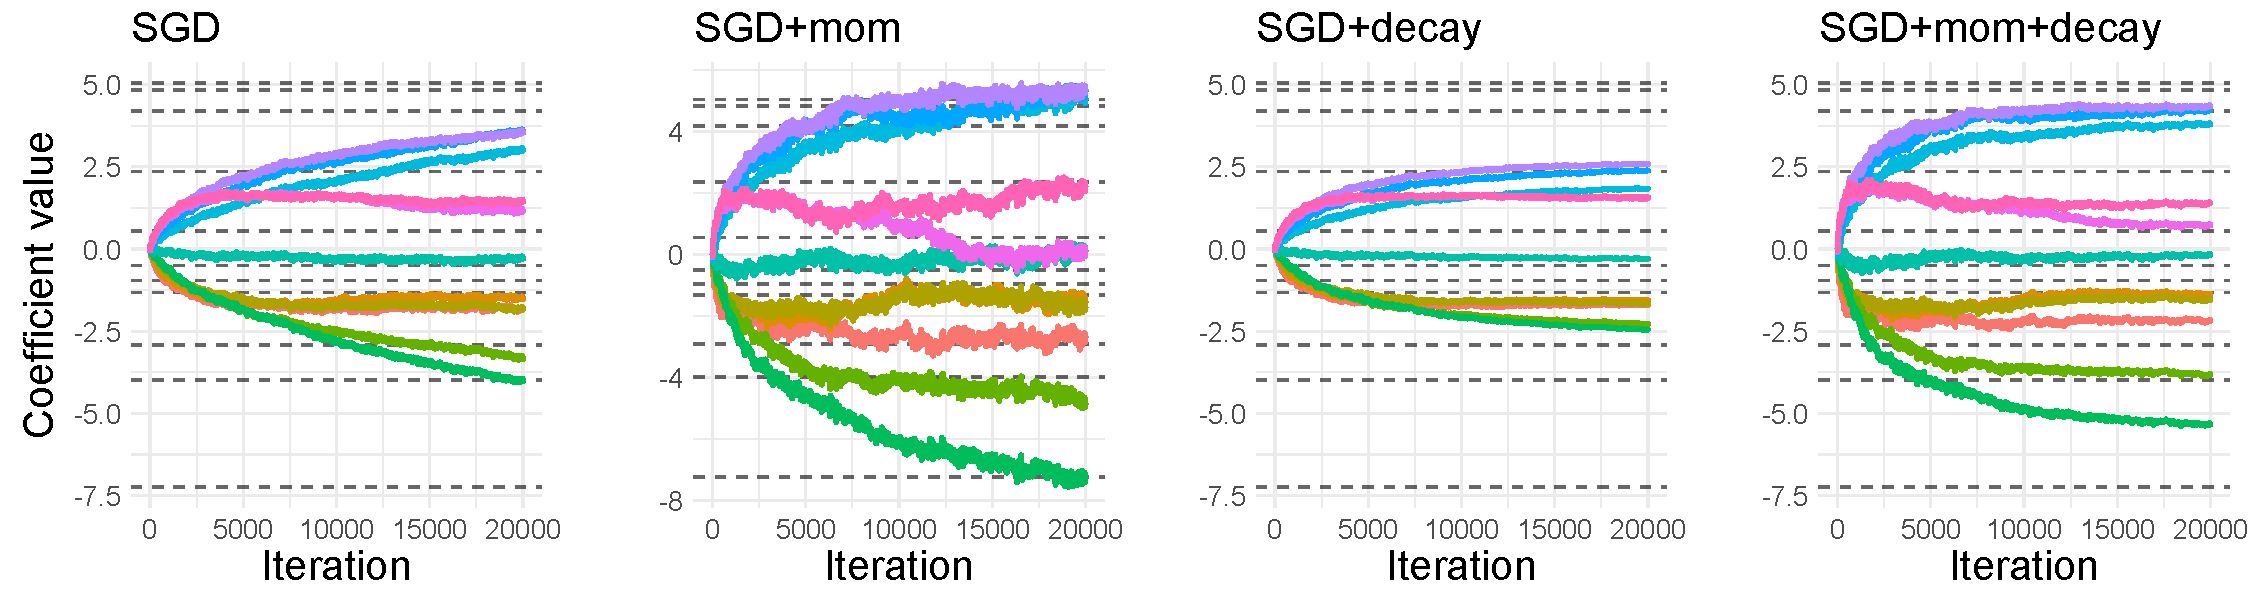
\includegraphics[width=0.8\textwidth]{figure_man/simu_linmod/SGD_log_coef_med_corr.pdf}\\
            \begin{footnotesize}
                %Dashed line in test loss indicates irreducible error due to $\sigma=1$
            \end{footnotesize}
\end{figure}
Only SGD and SGD+mom converge in $t_{\text{max}}=10000$. Decay slows down while momentum accelerates optim.
\end{vbframe}
\end{comment}

\begin{comment}
\begin{vbframe}{Log-Reg (SGD + small step size)}
\vspace{-0.4cm}
SGD with small $\alpha=3\cdot10^{-4}$ and indep. features:
\begin{figure}
            \includegraphics[width=0.8\textwidth]{figure_man/simu_linmod/SGD_log_small_lr_iters.pdf} \\
             \includegraphics[width=0.8\textwidth]{figure_man/simu_linmod/SGD_log_coef_small.pdf}\\
            \begin{footnotesize}
                %Dashed line in test loss indicates irreducible error due to $\sigma=1$
            \end{footnotesize}
\end{figure}
No method converges since lr is too small. Decay makes it even worse. 
\end{vbframe}
\end{comment}


\begin{vbframe}{Log-Reg (SGD + large step size)}
\vspace{-0.4cm}
SGD with large $\alpha=0.3$ and indep. features:
\begin{figure}
            \includegraphics[width=0.8\textwidth]{figure_man/simu_linmod/SGD_log_large_lr_iters.pdf} \\
             \includegraphics[width=0.8\textwidth]{figure_man/simu_linmod/SGD_log_coef_large.pdf}\\
            \begin{footnotesize}
                %Dashed line in test loss indicates irreducible error due to $\sigma=1$
            \end{footnotesize}
\end{figure}
\vspace{-0.2cm}
{\footnotesize
\textbf{High variance} in optim dynamics. Plain SGD and \textbf{Momentum} become unstable and oscillate at suboptimal loss values/diverge while \textbf{decay} (necessary to eliminate oscillations) performs best and is fastest. \textbf{Momentum+decay} initially diverges but recovers once step size reduces (would converge with many more steps).}
\end{vbframe}

%%%% DNN MNIST classification

\begin{vbframe}{Classification on MNIST (SGD)}
For a more realistic application, we compare optimizers on training an NN on subset of MNIST image classification task. 
\medskip
\begin{itemize}
     \setlength{\itemsep}{1.2em} 
    \item DNN has two hidden layers with $128$ and $64$ ReLU-activated units and Kaiming normal init. The loss is cross-entropy
    \item Instead of SGD we use mini-batch SGD with $100$ images per batch
    \item For the step size schedule, we use cosine decay $\alpha^{[t]} = \alpha^{[0]} \left[(1-r_{\text{min}}) \cdot \frac{1}{2}\left(1 + \cos\left(\pi \cdot \frac{t}{t_{\text{max}}}\right)\right) + r_{\text{min}}\right]$ with final step size fraction $r_{\text{min}}=0.01$
    \item In case of momentum we set the parameter to $0.8$
    \item Regular initial step size is $0.01$ and to $0.1$ for large step size
\end{itemize}
\end{vbframe}

\begin{vbframe}{Classification on MNIST (SGD)}
\vspace{-0.3cm}
Mini-batch SGD with $\alpha \in \{0.01, 0.1\}$ for 100 epochs (5000 iterations):
\begin{figure}
            \includegraphics[width=1.0\textwidth]{figure_man/simu_mnist/SGD_compar.pdf} \\
            %\begin{footnotesize}
            %    Irreducible error due to additive noise is $\sigma=1$
            %\end{footnotesize}
\end{figure}
\vspace{-0.2cm}
\textbf{Observations} 
{\footnotesize
(\textbf{NB}: \textcolor{green}{green}/\textcolor{cyan}{cyan} + \textcolor{blue}{blue}/\textcolor{magenta}{purple} train losses overlap but not val. acc.):\\ 
1. \textbf{Momentum} drastically speeds up optimization in all settings.\\
2. \textbf{Plain SGD}: step size decay slows optimization slightly. \\
3. SGD, SGD+cos and SGD+mom achieve \textbf{same} val. acc. \\
$\Rightarrow$ no generalization benefit for medium $\alpha$\\
4. \textbf{Cosine decay+momentum} improves generalization for medium $\alpha$ slightly. \\
5. \textbf{Large step size} with momentum and decay performs best}
\end{vbframe}

\begin{vbframe}{Classification on MNIST (GD vs. SGD)}
\vspace{-0.2cm}
Why is it not a good idea to use GD in most DL applications? SGD is much faster. Compare runtime of mini-batch SGD (batch size=$100$) with GD (constant $\alpha=0.01$ without momentum for $t_{\text{max}}=5000$ iterations):
\begin{figure}
            \includegraphics[width=1.0\textwidth]{figure_man/simu_mnist/SGD_GD_compar.pdf} \\
            %\begin{footnotesize}
            %    Irreducible error due to additive noise is $\sigma=1$
            %\end{footnotesize}
\end{figure} 
\textbf{Observations}:\\ 1. Mini-batch SGD is over an order of magnitude faster.\\
2. SGD generalizes better than GD despite being much faster. \\
\end{vbframe}



\endlecture
\end{document}

%%% 



%% 
